\chapter{Einleitung}

\section{Persönliche Motivation}
%Wenn jemanden etwas einfällt
%Persönlich! Was wollten wir cooles machen und warum
%Wo sind die Probleme bei diesen Mengen an Daten

Bei der Bearbeitung der Aufgabenstellung konnten wir feststellen, dass viele Punkte auch Raum für eine freie Gestaltung der Umsetzung lassen. Dadurch haben wir uns dazu entschlossen, in manchen Punkten auch einige für uns noch experimentelle Ansätze zu verfolgen bzw. zu erproben. Als Herausforderung haben wir es angesehen, die Entwicklung der Software unter einer einheitlichen Infrastruktur bei den unterschiedlich verwendeten Betriebssystemen der Studenten zur Verfügung stellen zu können. 

Zusätzlich stellt die Arbeit mit einem so großen Datensatz eine besondere Herausforderung dar, welche wir so bisher nicht in unserem Studium erfahren hatten. Die Verlagerung der Rechenarbeit auf das entfernte GPU-Labor der Hochschule war auch eine interessante Erfahrung.

\section{Datensatz}
%AK
Der Datensatz stammt von Open Legal Data, siehe \cite{openlegaldata}, und beinhaltet eine Sammlung von 104763 (Stand: Januar 2022) deutschen Gerichtsurteilen. Die Schöpfer hinter dieser Datensammlung haben es sich zur Aufgabe gemacht der Öffentlichkeit die Urteile frei zur Verfügung zu stellen. Normalerweise müssen Gerichtsurteile der Allgemeinheit zur Verfügung gestellt werden, da Gerichte im Interesse der Bevölkerung entscheiden sollen. Dies ist allerdings nicht oder teilweise nur spärlich der Fall.

\chapter{Infrastruktur}

\section{Docker}
%SP

Um bei jedem Studenten die Bibliotheken und Frameworks auf einer einheitlichen Infrastruktur gewährleisten zu können, haben wir alle Softwarebibliotheken in Docker Images eingepflegt. Durch den simplen Austausch der Konfigurationsdateien ist die Entwicklung der Software, wie in unserem Fall, auch auf unterschiedlichen Betriebssystemen möglich. Dabei wird das Backend, Frontend und die Datenbank jeweils als isolierte Applikation innerhalb der Containervisualisierung Docker betrieben. Durch eine zentrale Konfigurationsdatei der Container können diese einfach zwischen verschiedenen Entwicklungsumgebungen ausgetauscht und ausgeführt werden. Somit konnten wir sicherstellen, dass es zu keinen Problemen bei der Ausführung des Projektes auf unterschiedlichen Betriebssystemen, in unserem Fall Windows 10 und MacOS, kommt.

Bei der Konfiguration der einzelnen Images haben wir bereits existierende Images (Python, Node, Solr) aus dem offiziellen Docker Hub verwendet und diese mit unseren weiteren Anforderungen erweitert. Die einzelnen Komponenten werden in einer YAML-Datei konfiguriert, in welcher die Umgebungsvariablen sowie die unterschiedlichen Abhängigkeiten zwischen diesen Containern definiert werden. Mithilfe von Docker-Compose können diese dann schlussendlich auf dem Host-System gestartet werden.

\section{Architektur}
%HK

\begin{figure}[H]
 \centering
 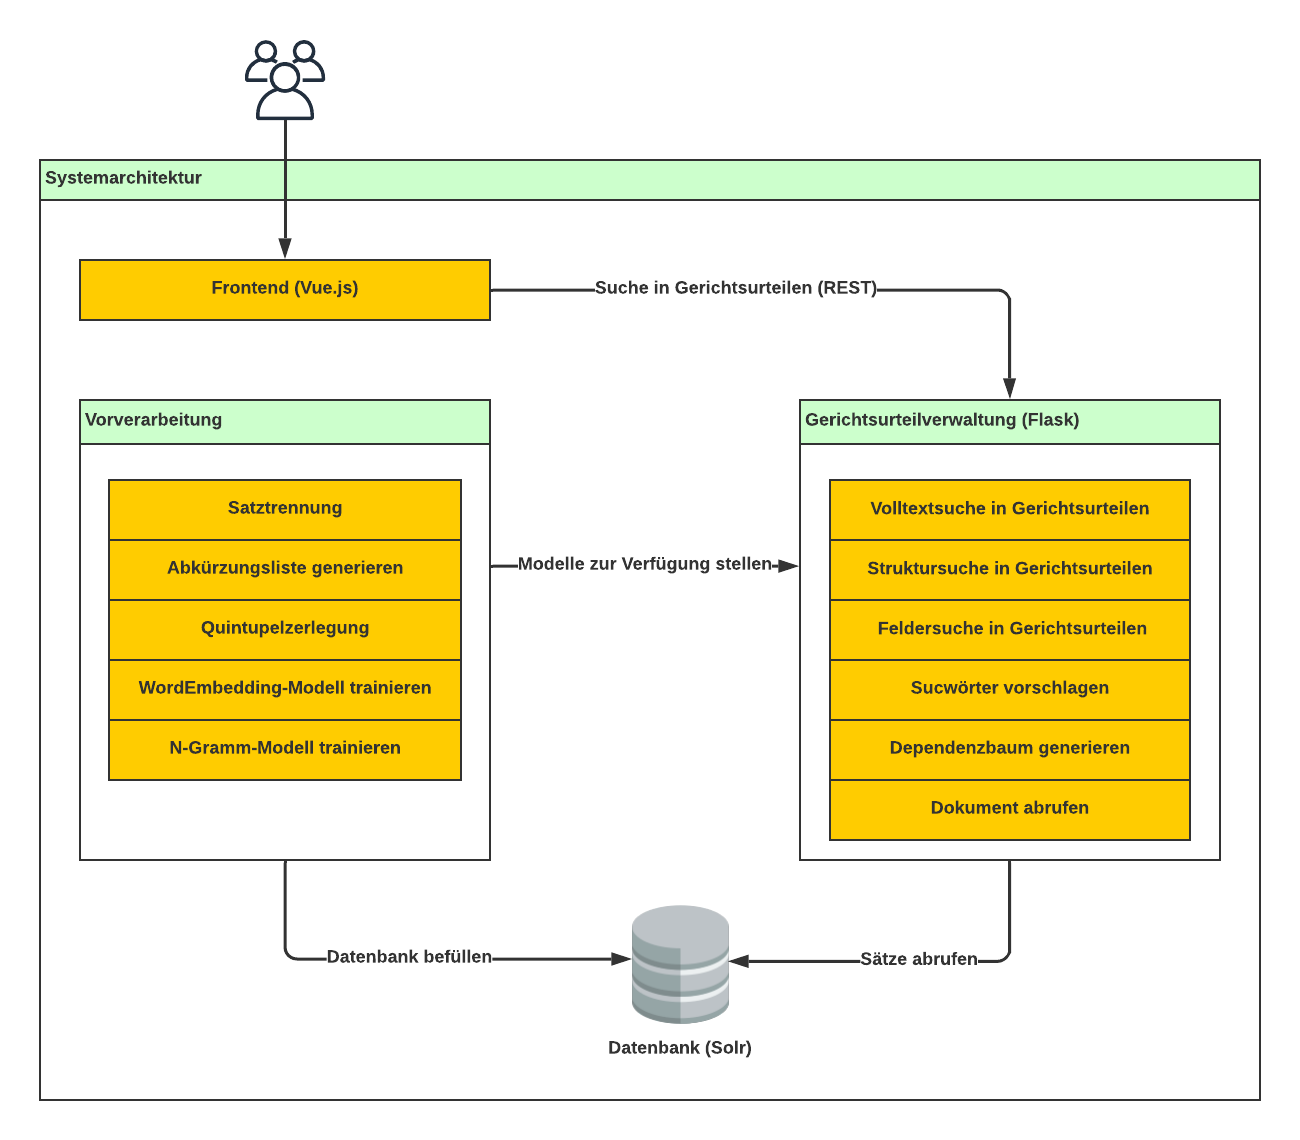
\includegraphics[width=\textwidth]{images/Systemarchitektur.png}
 \caption{Übersicht der Systemarchitektur}
 \label{fig:Systemarchitektur}
\end{figure}


\subsection{Frontend}
%SP
%- Vuetify
%- Node
%- Express
%- ...

\subsubsection{Node}

Bei der Entwicklung des Frontends haben wir uns dazu entschlossen, einen Node Server zu verwenden, da wir mit diesem die meiste Erfahrung besitzen. Er verwendet zur Implementation des Frontends als Single Page Application das Framework Vue Router. Zur Kommunikation mit dem Backend wird Axios verwendet.

\subsubsection{Vue}

Mithilfe von Vue ist es möglich, eine klare Trennung von JavaScript, HTML und CSS durchzuführen. In größeren Projekten wird somit bessere Übersichtlichkeit gewährleistet. Es existiert außerdem eine ausführliche und verständliche Dokumentation, die die Entwicklung mit diesem Framework erleichtert.

\subsubsection{Vuetify}

Dieses Framework bietet ähnlich zu Bootstrap viele weitere Komponenten, mit denen die Gestaltung der Benutzeroberfläche erleichtert wird. Zusätzlich kann es mit geringem Aufwand in eine Vue-Anwendung integriert werden. Beispielsweise bietet es die Möglichkeit, Daten bidirektional mit dem Model verknüpfen und auf Events reagieren zu können. Vuetify orientiert sich grundsätzlich am Material Design Standard.

\subsection{Backend}
%SP
%Flask

Der auf Python basierende Webserver Flask wird in unserer Anwendung als Backend-Server zur Kommunikation mit dem Frontend verwendet. Wir haben uns für Flask entschieden, da wir bis auf die Implementation des Frontends Python verwendet haben. Einkommende HTTP-Anfragen werden bearbeitet und mit JSON-Objekten beantwortet. Durch die Konzeption der Schnittstelle am REST-Standard könnte diese Komponente jederzeit durch eine auf einer anderen Technologie aufbauenden Komponente ersetzt werden, wenn die Schnittstellenrouten implementiert werden würden.

Der Backendserver bietet dabei die Möglichkeit, Anfragen nach Gesetzestexten an Solr weiterzuleiten beziehungsweise Suchvorschläge anhand der davor trainierten Modelle zu generieren. Dabei wird jeweils versucht, anhand der Modelle das jeweils nächste Wort vorherzusagen. Die Vorhersagen werden anschließend nach ihrer Wahrscheinlichkeit sortiert zurückgegeben.

Mithilfe von displacy, einem Submodul von SpaCy, generiert der Backendserver auf Anfrage für das Frontend einen Dependenzbaum.

\subsection{Solr}
%SP
%- Konfiguration des Servers
%- Felderdefinitionen
%- XML-Dateien
%- Struktur eines Feldes

Solr wird ebenso wie die anderen Komponenten innerhalb eines Docker Containers gestartet. Innerhalb dieses Containers wurde die Konfiguration des Cores  \glqq court-decisions\grqq{} abgelegt. Diese enthält die Konfiguration der einzelnen Datensätze, wie wir sie in der Datenbank speichern. Beim Start des Gesamtsystems wird die Datenbank vollautomatisch mit den aus der Vorbereitung generierten XML-Dateien, welche die Datensätze mit den extrahierten Quintupel enthält, befüllt. Somit entfällt der manuelle Konfigurationsaufwand der Felder und Import der Datensätze auf den einzelnen Host-Systemen komplett.

\begin{figure}[H]
 \centering
 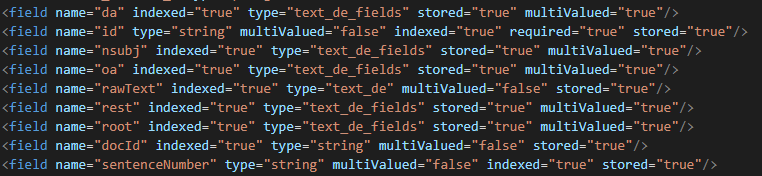
\includegraphics[width=\textwidth]{images/SolrSchema.png}
 \caption{Konfiguration der Felder}
 \label{fig:SolrSchema}
\end{figure}

Die Felder wurden zur schnelleren Suche indexiert und je nach Datentyp konfiguriert. Ebenso wurde definiert, ob innerhalb eines Feldes mehrere Werte zulässig sind. Als eindeutiger Schlüssel wird das Feld \glqq id\grqq{} verwendet, das eine Kombination der Werte \glqq docId\grqq{} und \glqq sentenceNumber\grqq{} aus den Gerichtsurteilen ist und im Vorbereitungsschritt in die zu importierenden XML-Dateien geschrieben wird. 

%# TODO? Stemming
\begin{figure}[H]
 \centering
 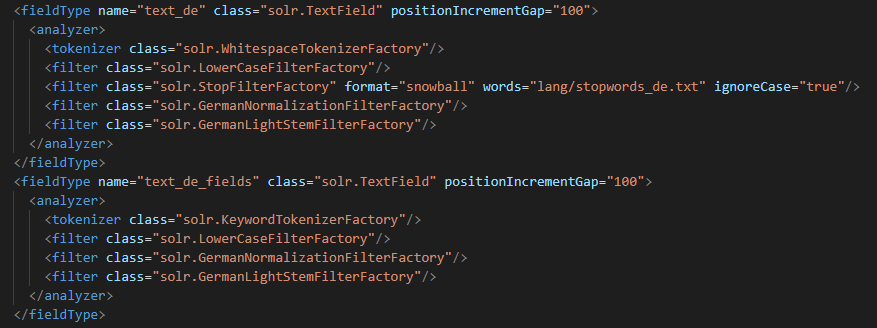
\includegraphics[width=\textwidth]{images/SolrFelderKonfigScreenshot.png}
 \caption{Konfiguration der Feldertypen}
 \label{fig:SolrSchema}
\end{figure}

Durch die Verwendung der Feldertypen text_de und text_de_fields, welche den Filter GermanLightStemFilterFactory verwenden, wurde die Stemmingfunktion von Solr auf diese Felder aktiviert. Dadurch werden bei der Rückgabe der Ergebnisse verschiedene morphologische Varianten eines Wortes beachtet. Der Unterschied der beiden Feldtypen ist dabei der Tokenizer. Die einzelnen Quintupel werden als Keyword-Tokens abgespeichert, während der Ursprungssatz selbst mit dem WhitespaceTokenizer behandelt wird. Dadurch wird es möglich in einem vollständigen Satz nach einem Datum zu suchen. Ohne wäre es nicht möglich beispielsweise nach dem \glqq 13. Februar\grqq{} zu suchen.


\chapter{Datenvorbereitung}
\section{Ablauf}
%SP+HK
%BILD?
%A=>B=>C
%Grundsätzliche Beschreibung des Ablaufs
%
% DO NOT ENTER TEXT HERE
%
\begin{figure}[H]
 \centering
 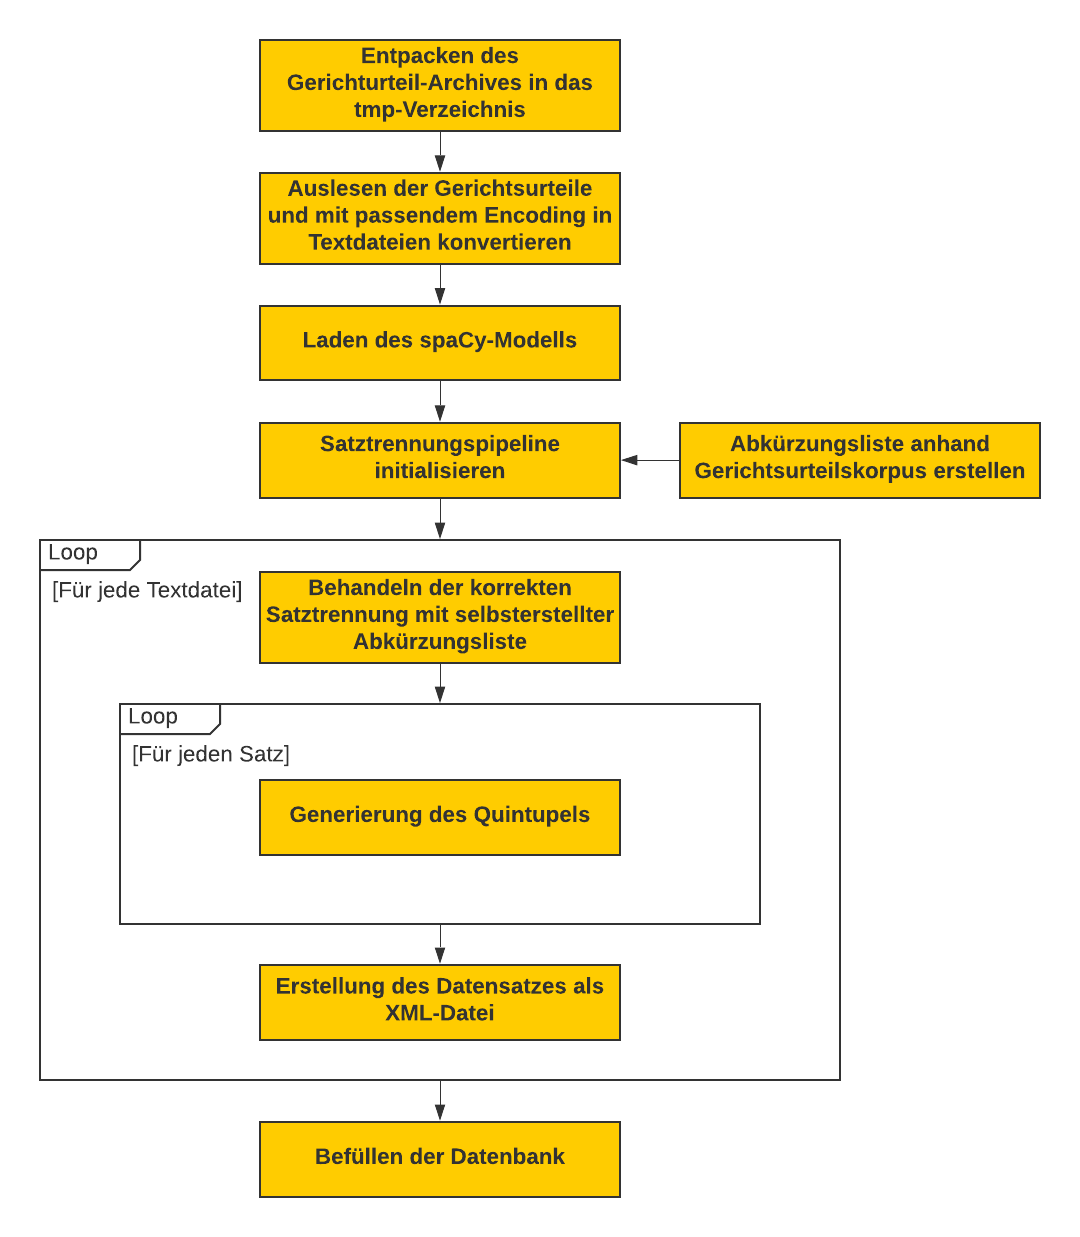
\includegraphics[width=0.75\textwidth]{images/AblaufDatenvorbereitung.png}
 \caption{Ablauf der Datenvorbereitung}
 \label{fig:AblaufDatenvorbereitung}
\end{figure}

\section{Satztrennung} \label{satztrennung}
%AK
%SBD
%- Abkürzungen
%- Zitations-Tags
%Satztrennung
Zur Datenvorbereitung werden die Texte in einzelne Sätze getrennt, da der Part-Of-Speech Tagger die Sätze für die korrekte Zuordnung der Satzteile benötigt. Das Problem der eingebauten Satztrennung von \textit{spacy} ist, dass diese keine oder nur wenige juristischen Abkürzungen kennt. Dadurch werden Sätze an den Stellen getrennt, die kein Satzende sind.

% Beispiel

\subsection{Abkürzungsliste}
Anhand des Datensatzes wurde eine Abkürzungsliste generiert. Dazu wurden die in \autoref{fig:RegexAusdruecke} dargestellten Regulärenausdruck entworfen, um möglichst viele Arten von Abkürzungsstilen zu finden. Aufgrund des Aufbaus der Regulärenausdruck werden auch Satzenden gefunden, also Wörter die keine Abkürzungen sind. Falls diese Wörter mit in die Liste eingefügt werden, würde dies zu einer Verfälschung der Ergebnisse führen.

\begin{figure}[h]
	\centering
	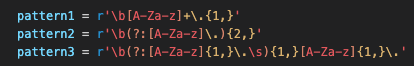
\includegraphics[keepaspectratio, width=0.75\textwidth]{RegexAusdruecke.png}
	\caption{Regex-Ausdrücke zum erkennen der Abkürzungen}
	\label{fig:RegexAusdruecke}
\end{figure}

Um diese Problematik zu umgehen, wurden die Regex-Ausrücke auf die einzelnen Dokumente angewendet und die Häufigkeit von den gefundenen Mustern ermittelt. Die entstandene Liste mit den Häufigkeiten wird der Größe nach sortiert und die häufigsten Abkürzungen stehen am Anfang der Liste. Diese Idee funktioniert, da man davon ausgehen kann, dass Wörter die mit einem Punkt enden häufiger eine Abkürzung sind als das gleiche Wort am Satzende. Mit steigender Anzahl von Dokumenten, wird dies auch genauer. In der Praxis klappt das nicht optimal und die Liste muss manuell überprüft und bearbeitet werden. Um das manuelle Bearbeiten zu erleichtern wurde zudem noch auf das Vokabular des Tiger-Corpus zurückgegriffen. Dadurch können vorab Wörter aussortiert werden, die in diesem Vokabular vorkommen.  In \autoref{fig:AbkuerzungshaeufigkeitsVerteilung} ist die Visualisierung der Abkürzungen zu sehen. Wenn die Häufigkeit der Wörter sinkt, dann lässt sich dort erkennen, dass das Verfahren ohne manuelles überprüfen nicht vollständig funktioniert. Mit dieser Methode lassen sich Abkürzungen abhängig von dem Datensatz anpassen.

\begin{figure}[h]
	\centering
	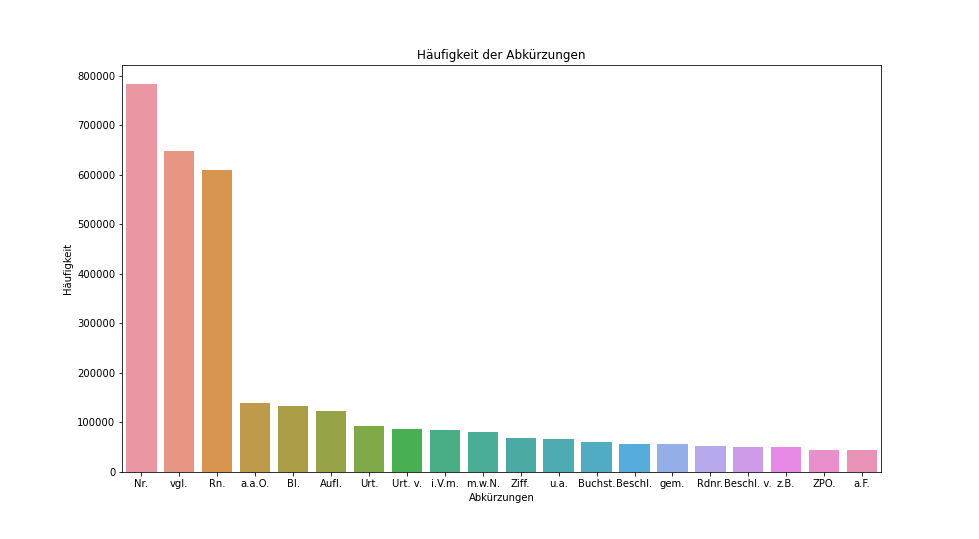
\includegraphics[keepaspectratio, width=\textwidth, height=\textheight]{AbkuerzungshaeufigkeitsVerteilung.png}
	\caption{Architektur U-Net}
	\label{fig:AbkuerzungshaeufigkeitsVerteilung}
\end{figure}

\subsection{Bibliothek PySBD}
Die manuell erstellte Abkürzungsliste auf den Datensatz ist nicht ausreichend um möglichst viele Fälle von unterschiedlichen Satzenden abzufangen. Die Python Bibliothek PySBD von \cite{sadvilkar-neumann-2020-pysbd} schafft Abhilfe. Dies ist ein Open-Source Paket, um Satzgrenzen zu erkennen. Durch das Einfügen dieser Funktion in die Pipeline wird dieser automatisch bei dem verarbeiten der einzelnen Dokumente angewendet und die fertigen Ergebnisse werden der Wortartbestimmung von \ref{quintupelbestimmung} übergeben. Besonders hervorzuheben ist, dass dieser deutlich bessere Ergebnisse auf den Texten liefert, wie der Standard Satzgrenzenerkenner von spacy.

\section{Quintupelbestimmung}\label{quintupelbestimmung}
%HK
%Quintupel mit dem Dependenparser
%Erzeugen / Finden
%- Conj-Strukuren (und-Verknüpfung von Satzteilen in nsubj, dobj, iobj) behandeln:
%z.B. verdoppeln von Einträgen oder in gleiches Feld mit einpacken (nicht automatisch in rest!)
Um die Wortarten zu bestimmen wird der Dependenzparser des Python-Moduls spaCy mit dem \glqq de_core_news_lg\grqq{}-Modell verwendet. Dafür werden, wie in Unterkapitel \ref{satztrennung} beschrieben, die Sätze eines Textes getrennt und satzweise verarbeitet.

Als erstes wird das Prädikat-Element eines Satzes als Wurzel ermittelt. Von diesem aus werden rekursiv alle Kinder bearbeitet und zu einem Quintupel-Objekt hinzugefügt. Das Quintupel-Objekt besteht aus den Teilen Prädikat, Subjekt, Akkusativ-Objekt (direktes Objekt), Dativ-Objekt (indirektes Objekt) und dem \glqq Rest\grqq{}.

Durch den rekursiven Algorithmus  werden Konjunktionsstrukturen so behandelt, dass mehrere Subjekte und Objekte in einem Satz identifiziert werden und somit auch im Quintupel vorhanden sind. Alle Satzteile, die nicht als Subjekt, Prädikat oder Objekt identifiziert werden, werden im Rest abgelegt.

\chapter{Modelle}
\section{Word-Embeddings}
%AK
% Funktion kurz
%- Wie trainiert Eigener Corpus, Gensim
Mithilfe der Bibliothek Gensim kann ein Modell auf einem eigenen Datensatz trainiert werden. Dazu muss diese Bibliothek installiert werden und mit den darin enthaltenen Funktionen der Corpus zum trainieren gebildet werden. Im letzten Schritt wird das Modell erstellt und mit den Daten trainiert. Im Trainingsvorgang wird ein hoch dimensionaler Vektor von jedem Wort gebildet. Mithilfe eines Ähnlichkeitsmaß wie der Kosinus-Ähnlichkeit kann der Unterschied zwischen 2 Wörtern berechnet werden. 

\section{N-Gramme}
%AK
% Funktion kurz
% Wie trainiert
Im Trainingsvorgang, wie in \autoref{fig:N_Gramme} dargestellt, werden die n Wortfolgen in dem zu zugrundeliegenden Datensatz gezählt und anschließend noch ein Alphabet mit allen vorkommenden Wörtern erstellt. Bei dem Vorhersagevorgang werden nun an dem eingegebenen n-1 langen Text nacheinander ein Wort aus dem Alphabet angehängt und mit der Liste der erstellten N-Gramme verglichen, ob diese Wortfolge existiert. Basierend auf der Häufigkeit wird als wahrscheinlichstes Ergebnis, die Folge mit dem höchsten Vorkommen gewählt. 

\begin{figure}[h]
	\centering
	
\includegraphics[keepaspectratio, width=0.5\textwidth]{N_Gramme.png}
	\caption{Trainingsvorgang der N-Gramme für N=3}
	\label{fig:N_Gramme}
\end{figure}

Aufgrund der großen Datenmenge mussten beim trainieren auf ständige Lese- und Schreibvorgänge von Dateien zurückgegriffen werden. Dies verlängert die Dauer des Trainingsvorgangs, aber somit kann der gesamte zur Verfügung stehende Datensatz genutzt werden. Ohne diese Methode ist es zu ständigen Abbrechens des Prozesses gekommen, da der Speicher zum halten der Datenmenge vollgelaufen ist.


\section{Unterschiede}
\begin{center}
	\begin{tabular}{|c c c c c|} 
		\hline
		\multicolumn{5}{|c|}{Trainingsresultate der Modelle} \\ [1ex] 
		\hline
		Modell & Epochen & Größe Vokabular & Trainingszeit & Vorhersagezeit \\ [0.5ex] 
		
		\hline
		NGrams & - &	+ NGram: 75365903 &  23 h & 1,16 s \\
		& &	+ Alphabet:  5478329&  & \\
		
		\hline
		NGrams &  - &	+ NGram:  1966682&  - & 0,37 s \\
		& &	+ Alphabet:  209894&  & \\
		
		\hline
		Word Embeddings & 5 & - & 30 min &  0,013 s \\
		
		\hline
		Word Embeddings & 50 & - & 4h &   0,011 s\\
		
		\hline
	\end{tabular}
\end{center}

\section{Implementierung}
In der Anwendung sind die beiden Modelle folgendermaßen implementiert. Beide Vorhersagen basieren auf einem unterschiedlichen Ansatz und aus diesem Grund ist es schwer eine Formel zu entwickeln, welche beide Ergebnisse zusammenfasst. Nachdem beide Modelle ein Wort vorhergesagt haben, werden die Ergebnisse der Größe nach der errechneten Wahrscheinlichkeit sortiert und die x wahrscheinlichsten Wörter angezeigt. 

\chapter{GUI}

\section{Suchen}
%SP+HK
%- Volltextsuche
%- Feldersuche
%- Struktursuche
%AJAX+AXIOS
\begin{figure}[H]
 \centering
 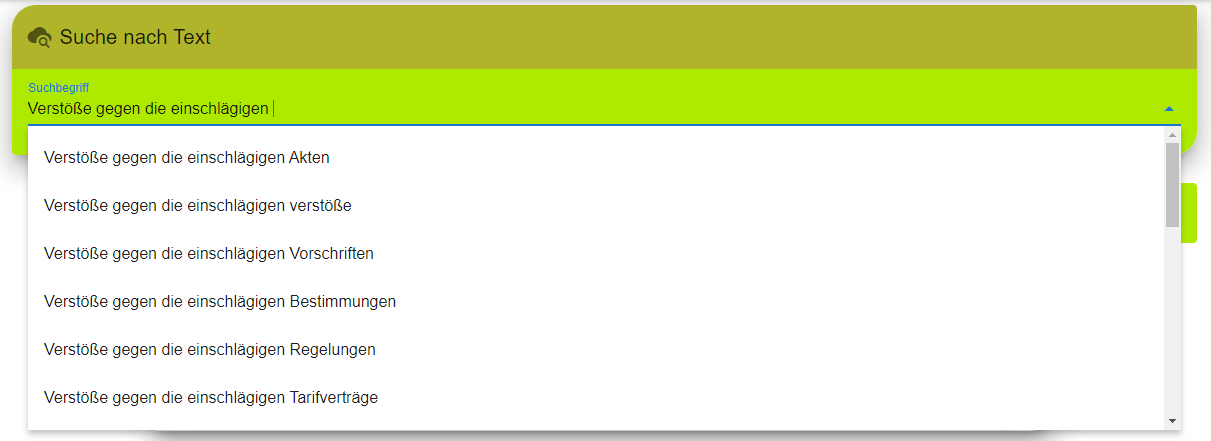
\includegraphics[width=\textwidth]{images/SucheScreenshot.png}
 \caption{Eingabe der Suche mit Suchvorschlägen}
 \label{fig:SucheScreenshot}
\end{figure}

\section{Suchergebnisse}
%SP+HK
%coole Funktionen
% ADD PAGINATION

Die Ausgabe der Suchergebnisse erfolgt als Liste. Zur besseren Übersicht und um das Laden von sehr vielen Daten zu unterbinden werden die Suchergebnisse zehn Elemente beschränkt. Weitere Ergebnisse lassen sich mithilfe der Navigation durch die Pagination nachladen. Diese enthält, neben dem gefundenen Satz, die zugehörige Dokument-ID und Satznummer zur Identifikation des Suchergebnisses und ermöglicht dem Nutzer das gewünschte Dokument zu finden. Zusätzlich finden sich in jedem Suchergebnis zwei Buttons, welche entweder den Dependenzbaum oder das vollständige Dokument anfordern und in einem neuen Fenster ausgegeben.

\begin{figure}[H]
 \centering
 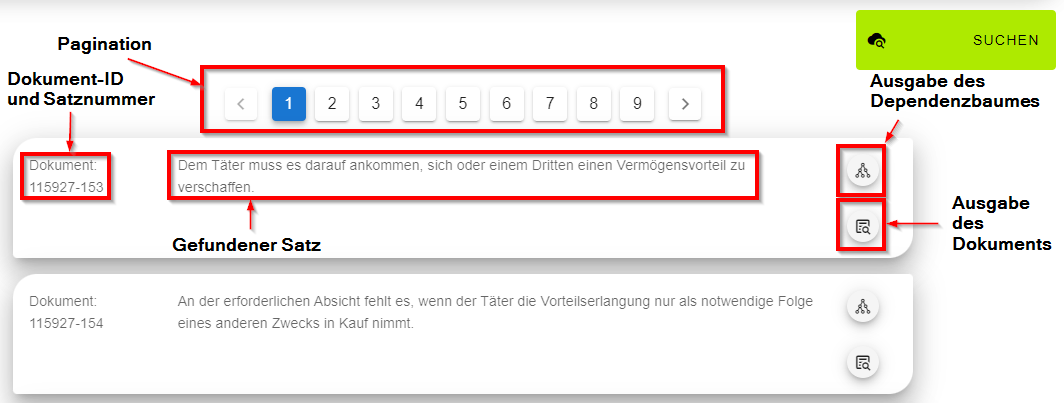
\includegraphics[width=\textwidth]{images/ResultScreenshot.png}
 \caption{Ausgabe der Ergebnisse}
 \label{fig:ResultScreenshot}
\end{figure}


Um den Dependenzbaum zu erstellen wird der gefundene Satz serverseitig erneut geparst und das Ergebnis als Baum gerendert und der Webanwendung zur Verfügung gestellt.

Fordert der Nutzer das Dokument an, so wird über die Dokument-ID jeder Satz des Dokuments aus der Datenbank abgerufen und zusammengefügt. Der gesuchte Satz wird zusätzlich markiert, um dem Nutzer die Suche im Dokument zu erleichtern.